% Options for packages loaded elsewhere
\PassOptionsToPackage{unicode}{hyperref}
\PassOptionsToPackage{hyphens}{url}
%
\documentclass[
]{article}
\usepackage{lmodern}
\usepackage{amssymb,amsmath,standalone}
\usepackage{ifxetex,ifluatex}
\ifnum 0\ifxetex 1\fi\ifluatex 1\fi=0 % if pdftex
  \usepackage[T1]{fontenc}
  \usepackage[utf8]{inputenc}
  \usepackage{textcomp} % provide euro and other symbols
\else % if luatex or xetex
  \usepackage{unicode-math}
  \defaultfontfeatures{Scale=MatchLowercase}
  \defaultfontfeatures[\rmfamily]{Ligatures=TeX,Scale=1}
\fi
% Use upquote if available, for straight quotes in verbatim environments
\IfFileExists{upquote.sty}{\usepackage{upquote}}{}
\IfFileExists{microtype.sty}{% use microtype if available
  \usepackage[]{microtype}
  \UseMicrotypeSet[protrusion]{basicmath} % disable protrusion for tt fonts
}{}
\makeatletter
\@ifundefined{KOMAClassName}{% if non-KOMA class
  \IfFileExists{parskip.sty}{%
    \usepackage{parskip}
  }{% else
    \setlength{\parindent}{0pt}
    \setlength{\parskip}{6pt plus 2pt minus 1pt}}
}{% if KOMA class
  \KOMAoptions{parskip=half}}
\makeatother
\usepackage{xcolor}
\IfFileExists{xurl.sty}{\usepackage{xurl}}{} % add URL line breaks if available
\IfFileExists{bookmark.sty}{\usepackage{bookmark}}{\usepackage{hyperref}}
\hypersetup{
  pdftitle={R Markdown Template},
  pdfauthor={Yingqi Jing},
  hidelinks,
  pdfcreator={LaTeX via pandoc}}
\urlstyle{same} % disable monospaced font for URLs
%%%\usepackage[margin=1in]{geometry}
%%\usepackage{color}
\usepackage{fancyvrb}
\newcommand{\VerbBar}{|}
\newcommand{\VERB}{\Verb[commandchars=\\\{\}]}
\DefineVerbatimEnvironment{Highlighting}{Verbatim}{commandchars=\\\{\}}
% Add ',fontsize=\small' for more characters per line
\usepackage{framed}
\definecolor{shadecolor}{RGB}{248,248,248}
\newenvironment{Shaded}{\begin{snugshade}}{\end{snugshade}}
\newcommand{\AlertTok}[1]{\textcolor[rgb]{0.94,0.16,0.16}{#1}}
\newcommand{\AnnotationTok}[1]{\textcolor[rgb]{0.56,0.35,0.01}{\textbf{\textit{#1}}}}
\newcommand{\AttributeTok}[1]{\textcolor[rgb]{0.77,0.63,0.00}{#1}}
\newcommand{\BaseNTok}[1]{\textcolor[rgb]{0.00,0.00,0.81}{#1}}
\newcommand{\BuiltInTok}[1]{#1}
\newcommand{\CharTok}[1]{\textcolor[rgb]{0.31,0.60,0.02}{#1}}
\newcommand{\CommentTok}[1]{\textcolor[rgb]{0.56,0.35,0.01}{\textit{#1}}}
\newcommand{\CommentVarTok}[1]{\textcolor[rgb]{0.56,0.35,0.01}{\textbf{\textit{#1}}}}
\newcommand{\ConstantTok}[1]{\textcolor[rgb]{0.00,0.00,0.00}{#1}}
\newcommand{\ControlFlowTok}[1]{\textcolor[rgb]{0.13,0.29,0.53}{\textbf{#1}}}
\newcommand{\DataTypeTok}[1]{\textcolor[rgb]{0.13,0.29,0.53}{#1}}
\newcommand{\DecValTok}[1]{\textcolor[rgb]{0.00,0.00,0.81}{#1}}
\newcommand{\DocumentationTok}[1]{\textcolor[rgb]{0.56,0.35,0.01}{\textbf{\textit{#1}}}}
\newcommand{\ErrorTok}[1]{\textcolor[rgb]{0.64,0.00,0.00}{\textbf{#1}}}
\newcommand{\ExtensionTok}[1]{#1}
\newcommand{\FloatTok}[1]{\textcolor[rgb]{0.00,0.00,0.81}{#1}}
\newcommand{\FunctionTok}[1]{\textcolor[rgb]{0.00,0.00,0.00}{#1}}
\newcommand{\ImportTok}[1]{#1}
\newcommand{\InformationTok}[1]{\textcolor[rgb]{0.56,0.35,0.01}{\textbf{\textit{#1}}}}
\newcommand{\KeywordTok}[1]{\textcolor[rgb]{0.13,0.29,0.53}{\textbf{#1}}}
\newcommand{\NormalTok}[1]{#1}
\newcommand{\OperatorTok}[1]{\textcolor[rgb]{0.81,0.36,0.00}{\textbf{#1}}}
\newcommand{\OtherTok}[1]{\textcolor[rgb]{0.56,0.35,0.01}{#1}}
\newcommand{\PreprocessorTok}[1]{\textcolor[rgb]{0.56,0.35,0.01}{\textit{#1}}}
\newcommand{\RegionMarkerTok}[1]{#1}
\newcommand{\SpecialCharTok}[1]{\textcolor[rgb]{0.00,0.00,0.00}{#1}}
\newcommand{\SpecialStringTok}[1]{\textcolor[rgb]{0.31,0.60,0.02}{#1}}
\newcommand{\StringTok}[1]{\textcolor[rgb]{0.31,0.60,0.02}{#1}}
\newcommand{\VariableTok}[1]{\textcolor[rgb]{0.00,0.00,0.00}{#1}}
\newcommand{\VerbatimStringTok}[1]{\textcolor[rgb]{0.31,0.60,0.02}{#1}}
\newcommand{\WarningTok}[1]{\textcolor[rgb]{0.56,0.35,0.01}{\textbf{\textit{#1}}}}
\usepackage{longtable,booktabs}
% Correct order of tables after \paragraph or \subparagraph
\usepackage{etoolbox}
\makeatletter
\patchcmd\longtable{\par}{\if@noskipsec\mbox{}\fi\par}{}{}
\makeatother
% Allow footnotes in longtable head/foot
\IfFileExists{footnotehyper.sty}{\usepackage{footnotehyper}}{\usepackage{footnote}}
\makesavenoteenv{longtable}
\usepackage{graphicx}
\makeatletter
\def\maxwidth{\ifdim\Gin@nat@width>\linewidth\linewidth\else\Gin@nat@width\fi}
\def\maxheight{\ifdim\Gin@nat@height>\textheight\textheight\else\Gin@nat@height\fi}
\makeatother
% Scale images if necessary, so that they will not overflow the page
% margins by default, and it is still possible to overwrite the defaults
% using explicit options in \includegraphics[width, height, ...]{}
\setkeys{Gin}{width=\maxwidth,height=\maxheight,keepaspectratio}
% Set default figure placement to htbp
\makeatletter
\def\fps@figure{htbp}
\makeatother
\setlength{\emergencystretch}{3em} % prevent overfull lines
\providecommand{\tightlist}{%
  \setlength{\itemsep}{0pt}\setlength{\parskip}{0pt}}
\setcounter{secnumdepth}{5}
\usepackage{textcomp}
\renewcommand{\thefigure}{S\arabic{figure}}
\renewcommand{\thetable}{S\arabic{table}}
\renewcommand{\thesection}{S\arabic{section}}
\renewcommand{\thesubsection}{S\arabic{section}.\arabic{subsection}}
\usepackage{tocloft}
\settowidth{\cftsecnumwidth}{S10x}
\usepackage{makecell}
\usepackage{booktabs}
\usepackage{longtable}
\usepackage{array}
\usepackage{multirow}
\usepackage{wrapfig}
\usepackage{float}
\usepackage{colortbl}
\usepackage{pdflscape}
\usepackage{tabu}
\usepackage{threeparttable}
\usepackage{threeparttablex}
\usepackage[normalem]{ulem}
\usepackage{makecell}
\usepackage{xcolor}
%%%% citation %%%%%
\usepackage{xpatch}
\usepackage[style=authoryear-comp, % compressed form (e.g., Gibson 1998, 2000)
	backend=biber,
	dashed=false, % avoid hide duplicated names in References
	sorting = none,
	maxcitenames=3,
	uniquelist=false, uniquename=false,
	maxbibnames=99]{biblatex}
\renewbibmacro{in:}{} % remove in: for journal articles in bibliography
\DeclareFieldFormat[article, inbook,incollection,inproceedings]{title}{#1} % remove the quotation for title in bibliography
\DeclareFieldFormat[thesis]{title}{\mkbibitalic{#1}}
\DeclareFieldFormat[article, inbook,incollection,inproceedings]{pages}{#1} %remove pp. in bibliography
\addbibresource{/Users/jakejing/switchdrive/bib/references.bib}

% 




%%%% load packages %%%%
\usepackage{gb4e}
\noautomath
\usepackage{standalone}
\usepackage{threeparttablex}
\usepackage{longtable}
\usepackage{amsmath}
\usepackage{caption}
\usepackage{subcaption}
\usepackage{upgreek}
\usepackage{float}
\usepackage{multirow}

%%%% define dimensions and margins %%%%
\usepackage[letterpaper,margin=1in]{geometry}

%%%% remove paragraph indentation globally %%%
\setlength{\parindent}{0pt}

% Keywords command
\providecommand{\keywords}[1]
{\small \textit{Keywords:} #1
}

\begin{document}
\thispagestyle{empty}

\begin{center}
%{\doublespacing
{\Large\sffamily\bfseries{R Markdown Template}
%}


{\normalsize Yingqi Jing}

}

{\large January 30, 2022}
\end{center}
\vspace{6pt}


\setcounter{footnote}{0}

%%%% abstract %%%%%%




\clearpage

\hypertarget{introduction}{%
\section{Introduction}\label{introduction}}

For large files, we can cache the file, and use \texttt{cache.lazy\ =\ T} to reuse the pre-computed results. To avoid overwriting the previously cached file, it is better to set the \texttt{cache=\ F}, when you want to use cachy.lazy to get the previously saved results. In this case, you do not need to cache the file again. You can also load the cached file, and check the environment to see whether the variables have already been saved.

If \texttt{cache\ =\ T}, knitr~will skip the execution of this code chunk if it has been executed before and nothing in the code chunk has changed since then. This is particularly useful when you want to reuse the figure (time-consuming). \textbf{When you modify the code chunk (e.g., revise the code or the chunk options), the previous cache will be automatically invalidated, and knitr will cache the chunk again.}

\begin{Shaded}
\begin{Highlighting}[]
\KeywordTok{print}\NormalTok{(}\StringTok{"Hello R markdown!"}\NormalTok{)}
\end{Highlighting}
\end{Shaded}

\begin{verbatim}
[1] "Hello R markdown!"
\end{verbatim}

\hypertarget{data-and-methods}{%
\section{Data and Methods}\label{data-and-methods}}

\begin{Shaded}
\begin{Highlighting}[]
\PreprocessorTok{#include }\ImportTok{<Rcpp.h>}
\KeywordTok{using} \KeywordTok{namespace}\NormalTok{ Rcpp;}
\CommentTok{// [[Rcpp::export]]}
\NormalTok{NumericVector timesTwo(NumericVector x) \{}
  \ControlFlowTok{return}\NormalTok{ x * }\DecValTok{2}\NormalTok{;}
\NormalTok{\}}
\end{Highlighting}
\end{Shaded}

\begin{Shaded}
\begin{Highlighting}[]
\KeywordTok{timesTwo}\NormalTok{(}\DecValTok{10}\NormalTok{) }\CommentTok{# test function in R chunk or console}
\end{Highlighting}
\end{Shaded}

\hypertarget{results}{%
\section{Results}\label{results}}

We can also save the plot as png files, by setting the dev = ``png'', and change the quality of the picture by setting dpi = 300.

Alternatively, you can convert all the saved pdfs into pngs with imagemagick in terminal:

convert -density 150 *.pdf -quality 100 -set filename:basename ``\%{[}basename{]}'' ``\%{[}filename:basename{]}.png''

\hypertarget{cross-reference-of-figures-tables-and-equations}{%
\subsection{Cross-reference of figures, tables and equations}\label{cross-reference-of-figures-tables-and-equations}}

We can also co-refer a plot in Figure \ref{fig:histogram-rng}. Pls avoid using underscore (\texttt{\_}) or white space in the co-reference labels. Likewise, you can also use \texttt{\textbackslash{}@ref(tab/eq:)} to refer to the specific table or equation. See Figure \ref{fig:CTMCgraphs}.

\begin{figure}
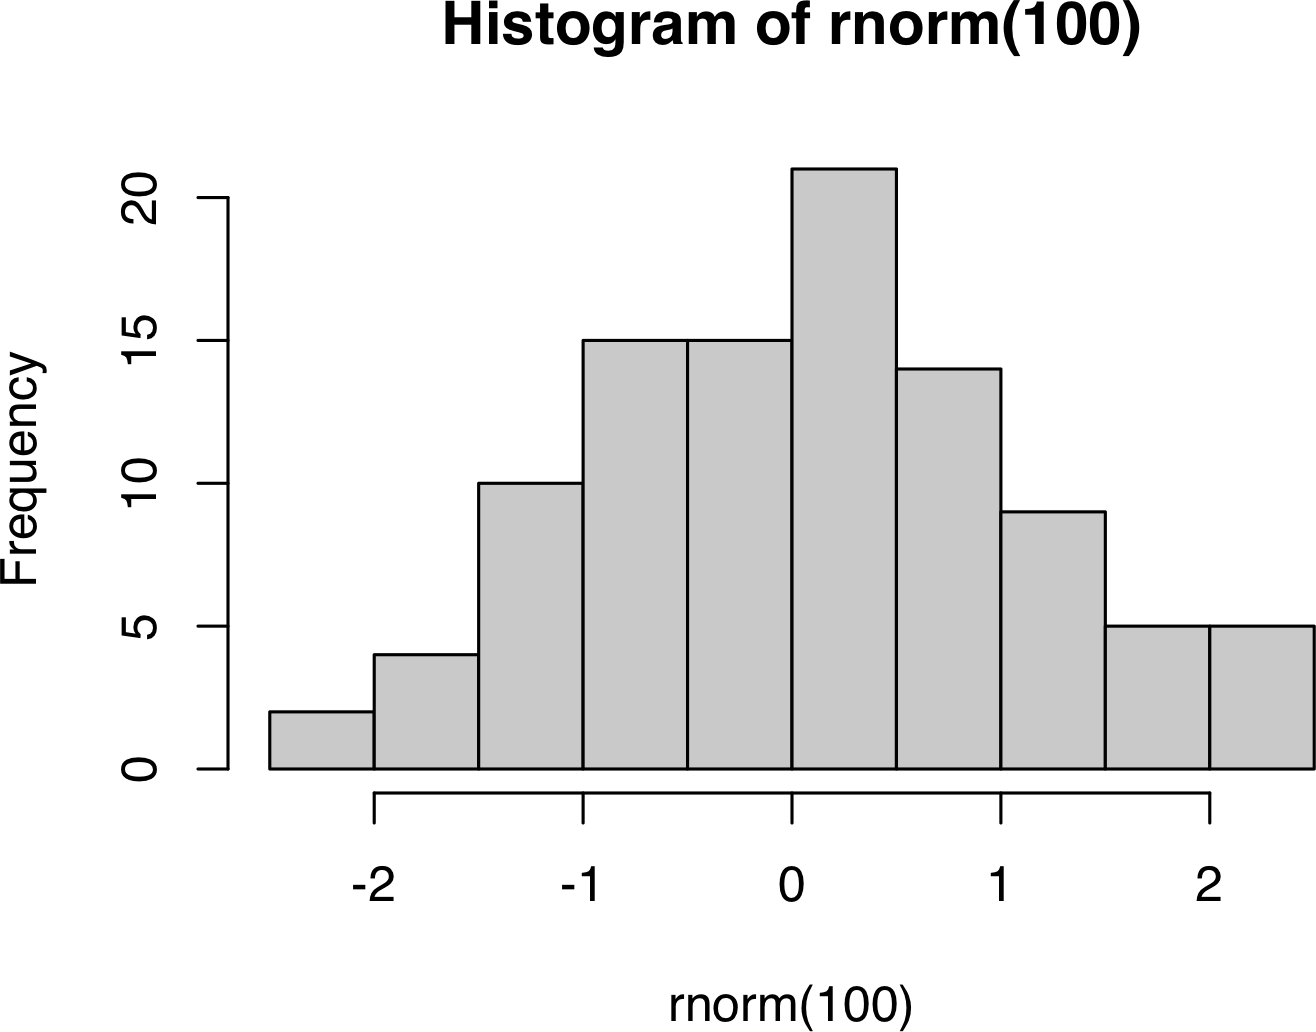
\includegraphics[width=1\linewidth,height=0.8\textheight]{./figures/histogram-rng-1} \caption{Histogram plot from \textcite{Rcore2020}}\label{fig:unnamed-chunk-3}
\end{figure}

\hypertarget{discussion}{%
\section{Discussion}\label{discussion}}

\begin{figure}
\centering
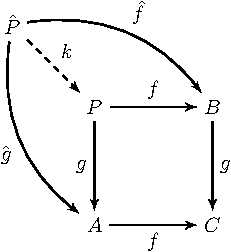
\includegraphics{figures/simpletikz-1.pdf}
\caption{\label{fig:simpletikz}Tikz graph example}
\end{figure}

\hypertarget{conclusions}{%
\section{Conclusions}\label{conclusions}}

\textbf{Note:} it seems that tikz does not support both fig.cap and fig.scap at the same time. It may cause fig.cap cannot recognize the latex code.

\begin{figure}

{\centering 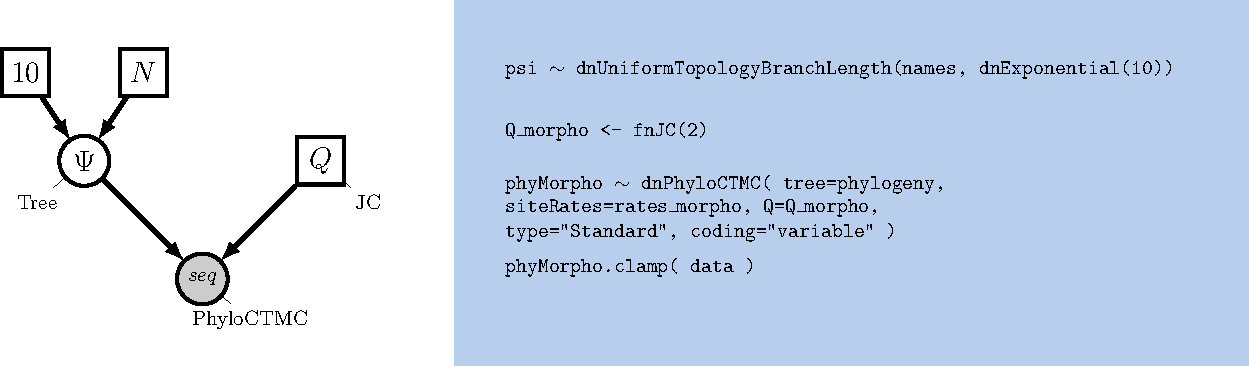
\includegraphics{figures/CTMCgraphs-1} 

}

\caption{A example graphs of CTMC model (fig.size cannot be changed via fig.width or fig.height)}\label{fig:CTMCgraphs}
\end{figure}

We can also add the cross-reference inside the figure cation via \texttt{\textbackslash{}\textbackslash{}ref\{fig:\}}.

\begin{figure}
\centering
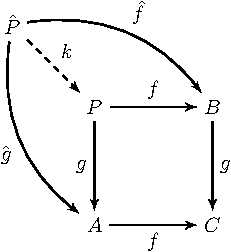
\includegraphics{figures/simpletikz-1.pdf}
\caption{\label{fig:simpletikz}A copy of CTMC model in Figure \ref{fig:histogram-rng} or Figure \ref{fig:histogram-rng} (reuse by its labels; doesn't work for read\_utf8)}
\end{figure}

\printbibliography[title=References]


\end{document}
